\documentclass[11pt,a4paper,titlepage]{article}
\usepackage[utf8]{inputenc}
\usepackage[margin=2cm,headheight=13.6cm]{geometry}
\usepackage{color}
% Agregados por mi
\usepackage{empheq}
\newcommand*\widefbox[1]{\fbox{\hspace{2em}#1\hspace{2em}}}
\usepackage{ifpdf}
\usepackage{hyperref}
\usepackage{booktabs}
\usepackage{amsmath}
\usepackage{mathtools}
\usepackage{amsfonts}
\usepackage{enumerate}
\usepackage{verbatim}
\usepackage{tikz}
\usetikzlibrary{shapes,snakes}
\newcommand*{\TitleParbox}[1]{\parbox[c]{3.75cm}{#1}}%
\newcommand*{\ntpb}[1]{\parbox[c]{3cm}{#1}}%
\usepackage{multicol}
\usepackage{cancel}
% Command "alignedbox{}{}" for a box within an align environment
% Source: http://www.latex-community.org/forum/viewtopic.php?f=46&t=8144
\newlength\dlf  % Define a new measure, dlf
\newcommand\alignedbox[2]{
% Argument #1 = before & if there were no box (lhs)
% Argument #2 = after & if there were no box (rhs)
&  % Alignment sign of the line
{
\settowidth\dlf{$\displaystyle #1$}  
    % The width of \dlf is the width of the lhs, with a displaystyle font
\addtolength\dlf{\fboxsep+\fboxrule}  
    % Add to it the distance to the box, and the width of the line of the box
\hspace{-\dlf}  
    % Move everything dlf units to the left, so that & #1 #2 is aligned under #1 & #2
\boxed{#1 #2}
    % Put a box around lhs and rhs
}
}

%Para el underbracket con el igual
\newlength\diz  % Define a new measure, diz
\newcommand\alignedunderbracket[2]{
% Argument #1 = before & if there were no box (lhs)
% Argument #2 = after & if there were no box (rhs)
&  % Alignment sign of the line
{
\settowidth\diz{$\displaystyle #1$}  
    % The width of \diz is the width of the lhs, with a displaystyle font
\addtolength\diz{\fboxsep+\fboxrule}  
    % Add to it the distance to the box, and the width of the line of the box
\hspace{-\diz}  
    % Move everything diz units to the left, so that & #1 #2 is aligned under #1 & #2
\underbracket{#1 #2}
    % Put a box around lhs and rhs
}
}


%Fin de agregados por mi
\usepackage{listings}
\usepackage{graphicx}
\usepackage[spanish]{babel}
\usepackage{caption}
\usepackage{float}
\usepackage{titling}
\usepackage{pgfkeys}
\definecolor{mygreen}{RGB}{0,127,0}
\definecolor{mygray}{RGB}{100,100,100}
\definecolor{mymauve}{RGB}{100,32,255}
\definecolor{lgray}{RGB}{230,230,230}
\lstset{ %
  frame=none,
  backgroundcolor=\color{white},   % choose the background color; you must add \usepackage{color} or \usepackage{xcolor}
  basicstyle=\footnotesize\ttfamily,        % the size of the fonts that are used for the code
  breakatwhitespace=false,         % sets if automatic breaks should only happen at whitespace
  breaklines=true,                 % sets automatic line breaking
  captionpos=t,                    % sets the caption-position to bottom
  commentstyle=\color{mygreen},    % comment style
  deletekeywords={...},            % if you want to delete keywords from the given language
  escapeinside={\%*}{*)},          % if you want to add LaTeX within your code
  extendedchars=true,              % lets you use non-ASCII characters; for 8-bits encodings only, does not work with UTF-8
%  frame=single,                    % adds a frame around the code
  keepspaces=true,                 % keeps spaces in text, useful for keeping indentation of code (possibly needs columns=flexible)
  keywordstyle=\color{blue},       % keyword style
  language=,                 % the language of the code
  morekeywords={*,...},            % if you want to add more keywords to the set
  numbers=left,                    % where to put the line-numbers; possible values are (none, left, right)
  numbersep=5pt,                   % how far the line-numbers are from the code
  numberstyle=\tiny\color{mygray}, % the style that is used for the line-numbers
  rulecolor=\color{black},         % if not set, the frame-color may be changed on line-breaks within not-black text (e.g. comments (green here))
  showspaces=false,                % show spaces everywhere adding particular underscores; it overrides 'showstringspaces'
  showstringspaces=false,          % underline spaces within strings only
  showtabs=false,                  % show tabs within strings adding particular underscores
  stepnumber=1,                    % the step between two line-numbers. If it's 1, each line will be numbered
  stringstyle=\color{mymauve},     % string literal style
  tabsize=4,                       % sets default tabsize to 2 spaces
  aboveskip=3mm,
  belowskip=3mm,
}

\usepackage{fancyhdr}
\pagestyle{fancy}
\rhead{High Level Synthesis con Vivado}
\usepackage{datetime}
\usepackage{moresize}

\newdateformat{monthyeardate}{%
  \monthname[\THEMONTH] \THEYEAR}

\newcommand{\rulebreak}{%
	\par%
	\vspace{0.9cm}%
    \noindent\rule{4cm}{0.4pt}%
    \vspace{1.2cm}%
    \par%
}

\newcommand{\coverpage}[1]{%
	\pagenumbering{roman}%
	\thispagestyle{empty}%
	\lhead{\textsc{\small{High Level Synthesis using Vivado HLS–} #1}}%
    \title{ESE}%
    \author{Leandro Marsó}%
    \newgeometry{left=5cm,bottom=2cm,right=5cm,top=2cm}%
	\begin{center}\hspace{0pt}\vfill%
    \uppercase{
    Universidad Nacional de San Luis \\
    Facultad de Ciencias Físico Matemáticas y Naturales
    }
	\rulebreak%
    {\Large\textbf{Tema}}
    
    \vspace{0.5cm}
    {\HUGE\textbf{\textit{#1}}}
    
    \vspace{0.5cm}
	\theauthor%
	\par%
	\vspace{0.9cm}%
    \noindent\rule{4cm}{0.4pt}%
    \vspace{0.45cm}
    \tableofcontents%
	\rulebreak%
    \monthyeardate\today\par
    \hspace{0pt}
	\end{center}%
    \vfill
    \hspace{0pt}
	\pagebreak%
    \restoregeometry%
    \pagenumbering{arabic}%
}

% Custom arguments for /fig command
\pgfkeys{
 /fig/.is family, /fig,
 default/.style = 
  {scale = 1,
   angle = 0},
 scale/.estore in = \figScale,
 angle/.estore in = \figAngle
}
\newcommand{\fig}[2][]{%
	\pgfkeys{/fig, default, #1}%
	\begin{figure}[H]%
    \centering
    \includegraphics[angle=\figAngle,width=\figScale\textwidth]{#2}%
	\end{figure}%
}

\newcommand{\filename}[1]{%
	\texttt{#1}%
}

\newcommand{\codigoc}[1]{%
  \lstinputlisting[language=c]{#1}
}

\newcommand*\paths[1]{\lstset{inputpath=#1}\graphicspath{#1}}


\everymath{\displaystyle} %Esto es para que la matemática dentro de texto sea más grande que el texto
\begin{document}
\coverpage{Pseudo Random Binary Sequence con Vivado HLS}

\section{Introducción}
En el presente informe, mostraremos los resultados de utilizar la herramienta de síntesis de alto nivel, aplicada a un código fuente en C. El circuito que queremos implementar es un generador de PRBS (Pseudo Random Binary Sequence). Implementamos una PRBS de 31.

\section{Implementación}
\paragraph{PRBS31}
En este caso, el polinomio generador que usamos es el siguente:
\begin{equation*}
\mbox{PRBS7} = x^{31} + x^{28} + 1
\end{equation*}
Y el código fuente a sintetizar es el siguiente
\begin{lstlisting}
#include "prbs31.h"

void prbs31(result_t * hw_out) {
    static data_t a = SEED;
        int newbit = (((a >> 30) ^ (a >> 27)) & 1);
        a = ((a << 1) | newbit) & 0x7fffffff;
        *hw_out = a;
    }
\end{lstlisting}
Cuyo archivo de definiciones es:
\begin{lstlisting}
#ifndef _PRBS31_H
#define _PRBS31_H
#define SEED 0x02
typedef int data_t;
typedef int result_t;
void prbs31(result_t * out);
#endif
\end{lstlisting}

En el \emph{testbench} del circuito hemos calculado por software la misma función y comparado con lo que devuelve la función a sintetizar. Ademas, declaramos una condición de finalización de la simulación, ya una PRBS una vez terminado el ciclo, vuelve a repetir todos los valores. Declaramos que pare en la iteración 1000 aproximadamente.

\paragraph{Resultado de la síntesis} El primer aspecto a resaltar es la performance de este circuito. Vemos en la figura \ref{fig:performance31} que la latencia es un ciclo de clock, y se estima que el período del mismo puede ser $1.37ns$

\begin{figure}[!h]
\centering
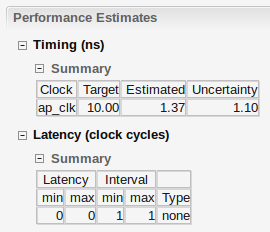
\includegraphics[height=4.5cm]{figuras/performancePRBS31}
\caption{Velocidad del clock y latencia}
\label{fig:performance31}
\end{figure}

Sobre los recursos utilizados, el reporte de la figura \ref{fig:utilization31} nos muestra 32 flip flops y una LUT (que implementa la semi-suma). Esto nos muestra que la implementación de la PRBS si hizo muy eficientemente, ya que si lo hubíesemos descripto en algún HDL, esperáriamos 31 FF y una XOR.
 
\begin{figure}[!h]
\centering
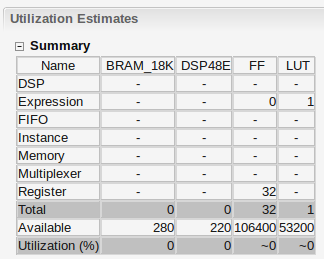
\includegraphics[height=4.9cm]{figuras/utilizationPRBS31}
\caption{Recursos utilizados}
\label{fig:utilization31}

\end{figure}

Sobre los puertos creados para el circuito, vemos en la figura \ref{fig:registersAndPortsPRBS31} el clock, reset, y otras señales auxiliares, además del puerto \emph{hw\_out} de salida de nuestro circuito.

\begin{figure}[!h]
\centering
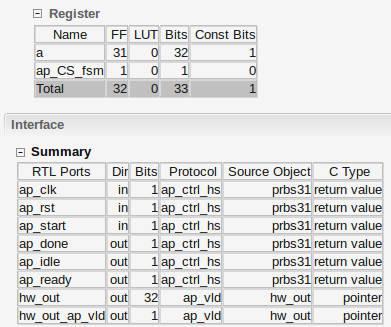
\includegraphics[height=6.2cm]{figuras/registersAndPortsPRBS31}
\caption{Puertos y registros}
\label{fig:registersAndPortsPRBS31}
\end{figure}

Resumimos en la tabla \ref{tab:resumen31} los resultados de esta síntesis:
\begin{table}[!h]
\centering
\caption{Resumen}
\label{tab:resumen31}
\begin{tabular}{@{}lccccc@{}}
\toprule
Puerto & Descripción\\ \midrule
Estimated clock period  & 1.37ns     \\ \midrule
Worst case latency &  1 \\\midrule
Number of FFs used: & 32\\\midrule
Number of LUTs used: & 1 \\\bottomrule
\end{tabular}
\end{table}

\section{Simulación}

Por último, hacemos una co-simulación con el RTL sintetizado para asegurarnos que todo está bien:
\begin{figure}[!h]
\centering
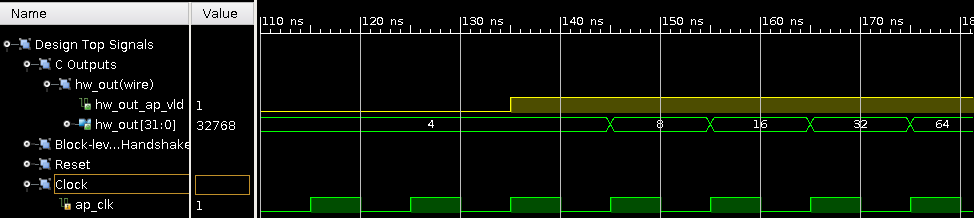
\includegraphics[width=0.8\textwidth]{figuras/waveform-prbs31}
\caption{Simulación del RTL}
\label{fig:waveform-prbs31}
\end{figure}
\section{Optimizaciones}
Por el tipo de circuito elegido, encontramos que no hay optimización alguna que se pueda realizar en este nivel del flujo de diseño, ya que el resultado de la primera síntesis nos brinda un bloque que resuelve el cálculo en un ciclo de reloj.

\section{Conclusión}
Partiendo del código fuente en C del circuito, hemos utilizado la herramienta de síntesis HLS de Vivado, con un resultado óptimo en la primera corrida. También hemos implementado una PRBS7 (no incluida en el informe por tener resultados análogos) con mucha facilidad y reutilizando el testbench. Por lo que pudimos ver que este flujo de diseño nos permite el desarrollo rápido de hardware utilizando conceptos de programación imperativa.

\end{document}
\paragraph{PRBS7}
Utilizaremos el siguiente polinomio generador:
\begin{equation*}
\mbox{PRBS7} = x^7 + x^6 + 1
\end{equation*}

Código fuente a sintetizar:

\paragraph{Código fuente en C}
\begin{lstlisting}
#include "prbs7.h"

void prbs7(result_t * hw_out) {
    static data_t a = SEED;
        int newbit = (((a >> 6) ^ (a >> 5)) & 1);
        a = ((a << 1) | newbit) & 0x7f;
        *hw_out = a;
    }
}
\end{lstlisting}


Usamos las siguientes definiciones:
\begin{lstlisting}
#ifndef _PRBS7_H
#define _PRBS7_H
#define SEED 0x02
typedef short   data_t;
typedef short result_t;
void prbs7(result_t * out);
#endif
\end{lstlisting}


